\documentclass[tikz,border=5mm]{standalone}
\usepackage[utf8]{vietnam}
\usetikzlibrary{calc}
\definecolor{nentrai}{RGB}{243, 212, 183}
\definecolor{nengiua}{RGB}{252, 225, 204}
\definecolor{chi}{RGB}{145, 61, 77}
\definecolor{mauvodam}{RGB}{59, 4, 9}
\definecolor{mauvosang}{RGB}{253, 205, 203}
\begin{document} 
	\begin{tikzpicture}[scale=2]
		\path (0,0) node[opacity=0,scale=.5,xscale=1]{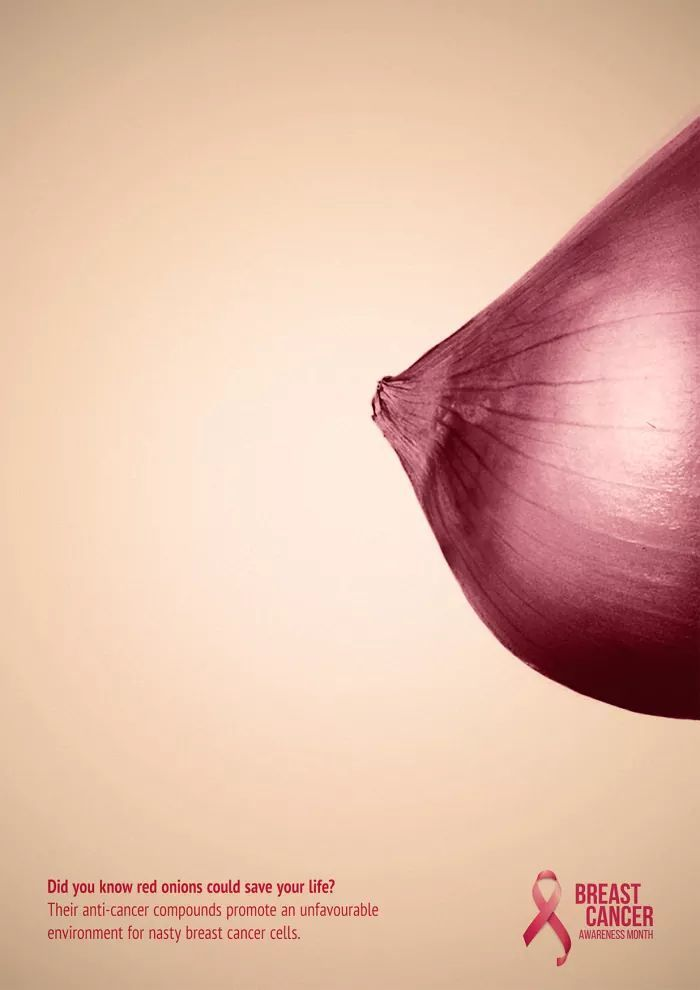
\includegraphics{onion.jpg}};
		\begin{pgfinterruptboundingbox}
			\shade[shading=radial,
			color= nentrai,
			outer color= nengiua,
			inner color=white!20] 
			(-3.08,-4.35)rectangle(3.08,4.35) ;
			\shade[shading=radial,
			color= mauvodam!20,
			outer color= mauvodam!80,
			inner color=red!70] 
			(3.08,-2) 
			..controls +(179:2.2)and +(-40:.6)..(.19,.7)[bend right]--(.2,.9) 
			..controls +(80:.15)and +(-150:.1)..(.3,1.05)--(.42,1.05) 
			..controls +(40:.25)and +(-130:.9)..(3.08,3.35) --(3.08,-2);
			\draw[chi,line width=.1pt]
			(.8,1) 
			..controls +(15:1)and +(180:1)..(3.08,1.6) 
			(1,.82) 
			..controls +(-12:1.3)and +(180:1)..(3.08,.54) 
			(.8,.9) 
			..controls +(-35:1)and +(175:.9)..(3.08,0) 
			(3.08,0) coordinate 
			..controls +(-35:1)and +(175:1.2)..(3.08,-.55) ;
			%\node at (-1,-2) [purple,rotate=-0]{NGUYỄN CÁT TUÒNG};
		\end{pgfinterruptboundingbox}
	\end{tikzpicture}

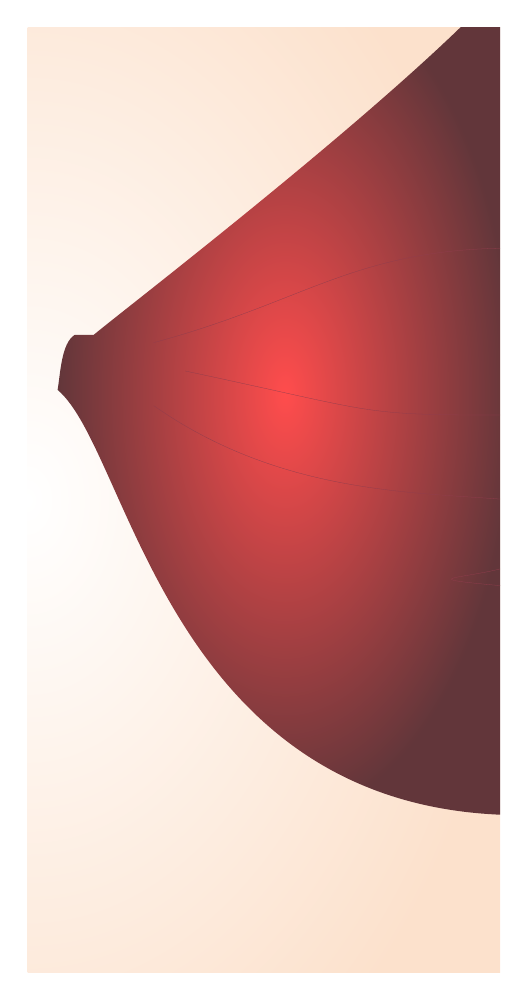
\begin{tikzpicture}[scale=2]
	\clip (0,-3) rectangle +(3,6);
	\shade[shading=radial,color= nentrai,outer color= nengiua,inner color=white!20]
	(-3.08,-4.35)rectangle(3.08,4.35) ;
	\shade[shading=radial,color= mauvodam!20,outer color= mauvodam!80,inner color=red!70]
	(3.08,-2) ..controls +(179:2.2)and +(-40:.6)..(.19,.7)[bend right]--(.19,.7)
	..controls +(80:.1)and +(-150:.1)..(.3,1.05)--(.42,1.05)
	..controls +(40:.25)and +(-130:.9)..(3.08,3.35) --(3.08,-2);
	\draw[chi,line width=.1pt](.8,1)
	..controls +(15:1)and +(180:1)..(3.08,1.6)
	(1,.82) ..controls +(-12:1.3)and +(180:1)..(3.08,.54)
	(.8,.6) ..controls +(-35:1)and +(175:.6)..(3.08,0)
	(3.08,0) ..controls +(-35:1)and +(175:1.2)..(3.08,-.55) ;
\end{tikzpicture}
\end{document}